\subsection{Systematic uncertainty}
\label{sec:Syst}

\begin{figure}[t]
\begin{center}
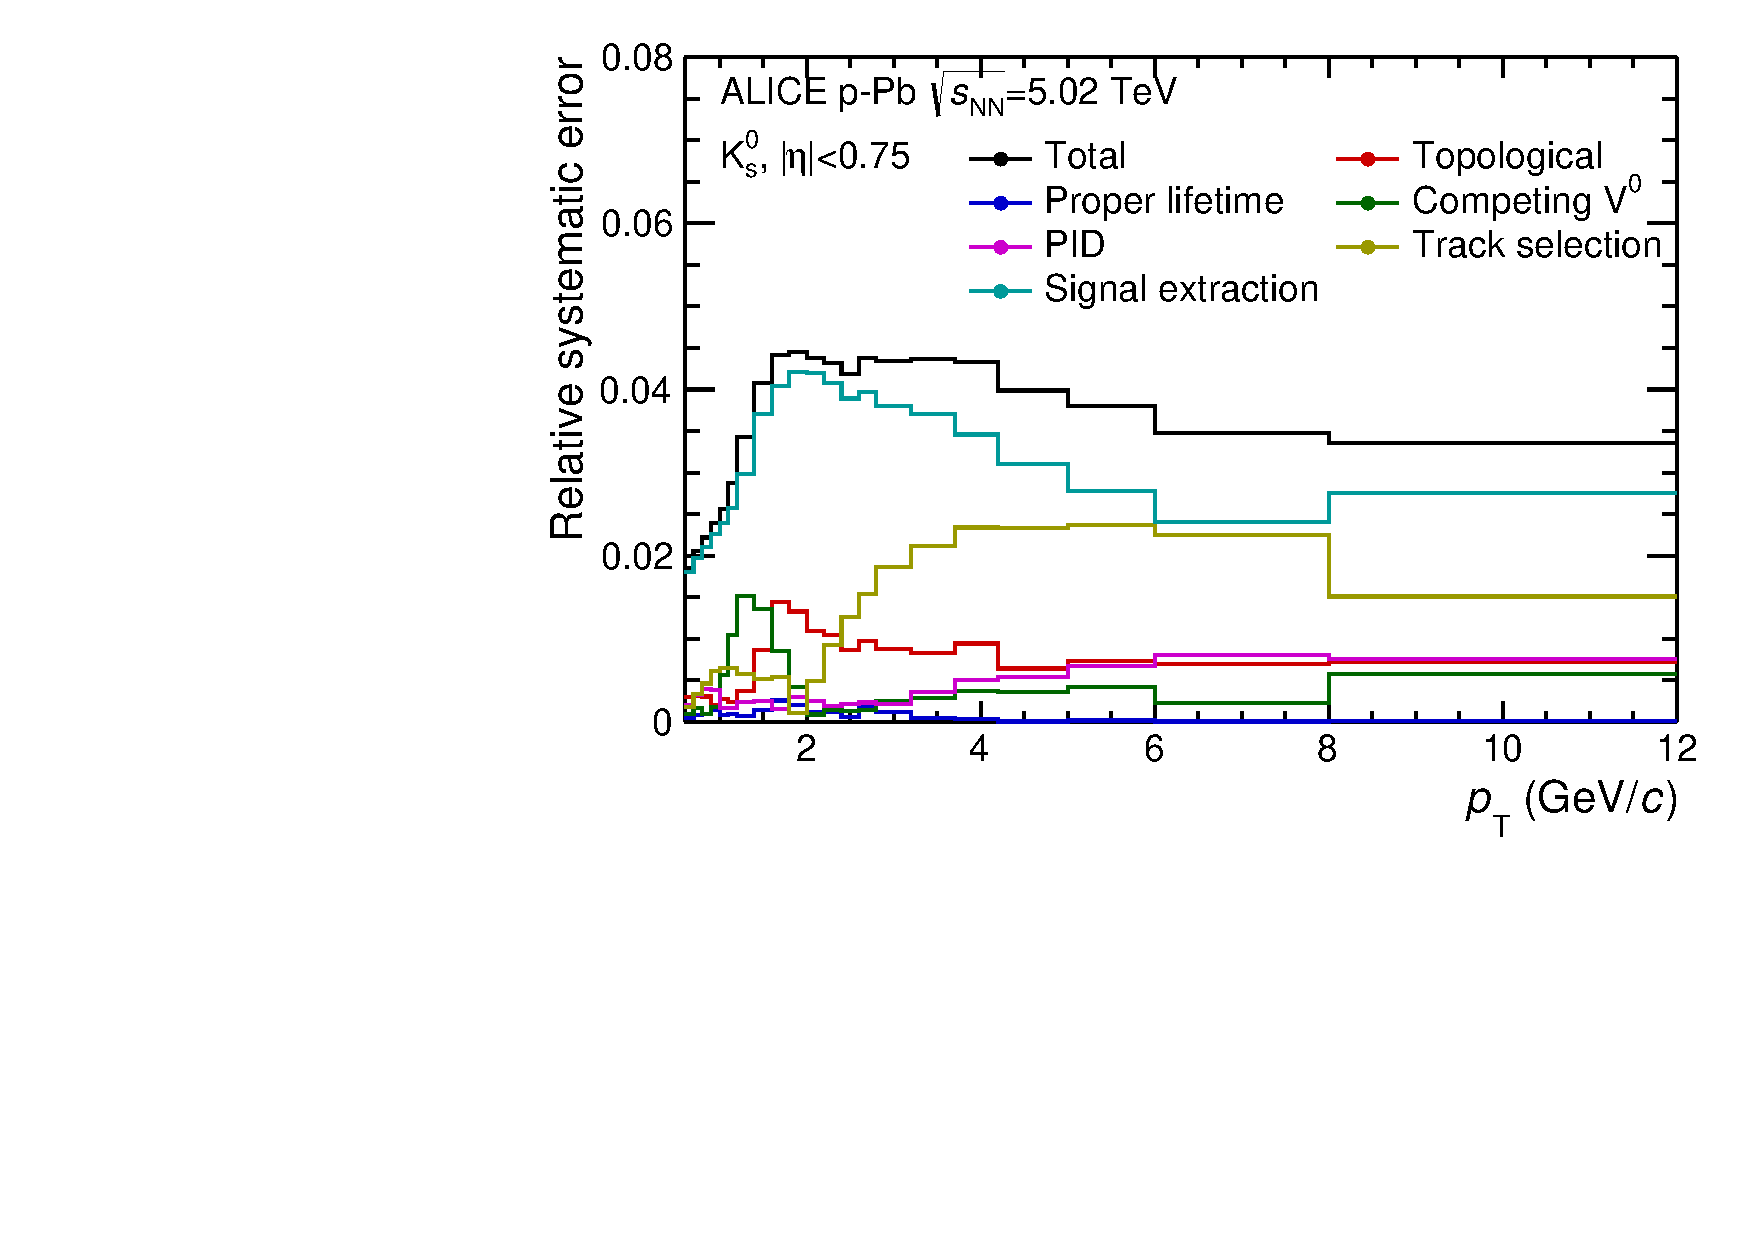
\includegraphics[width=.32\textwidth]{cSystIncl_Kshort}
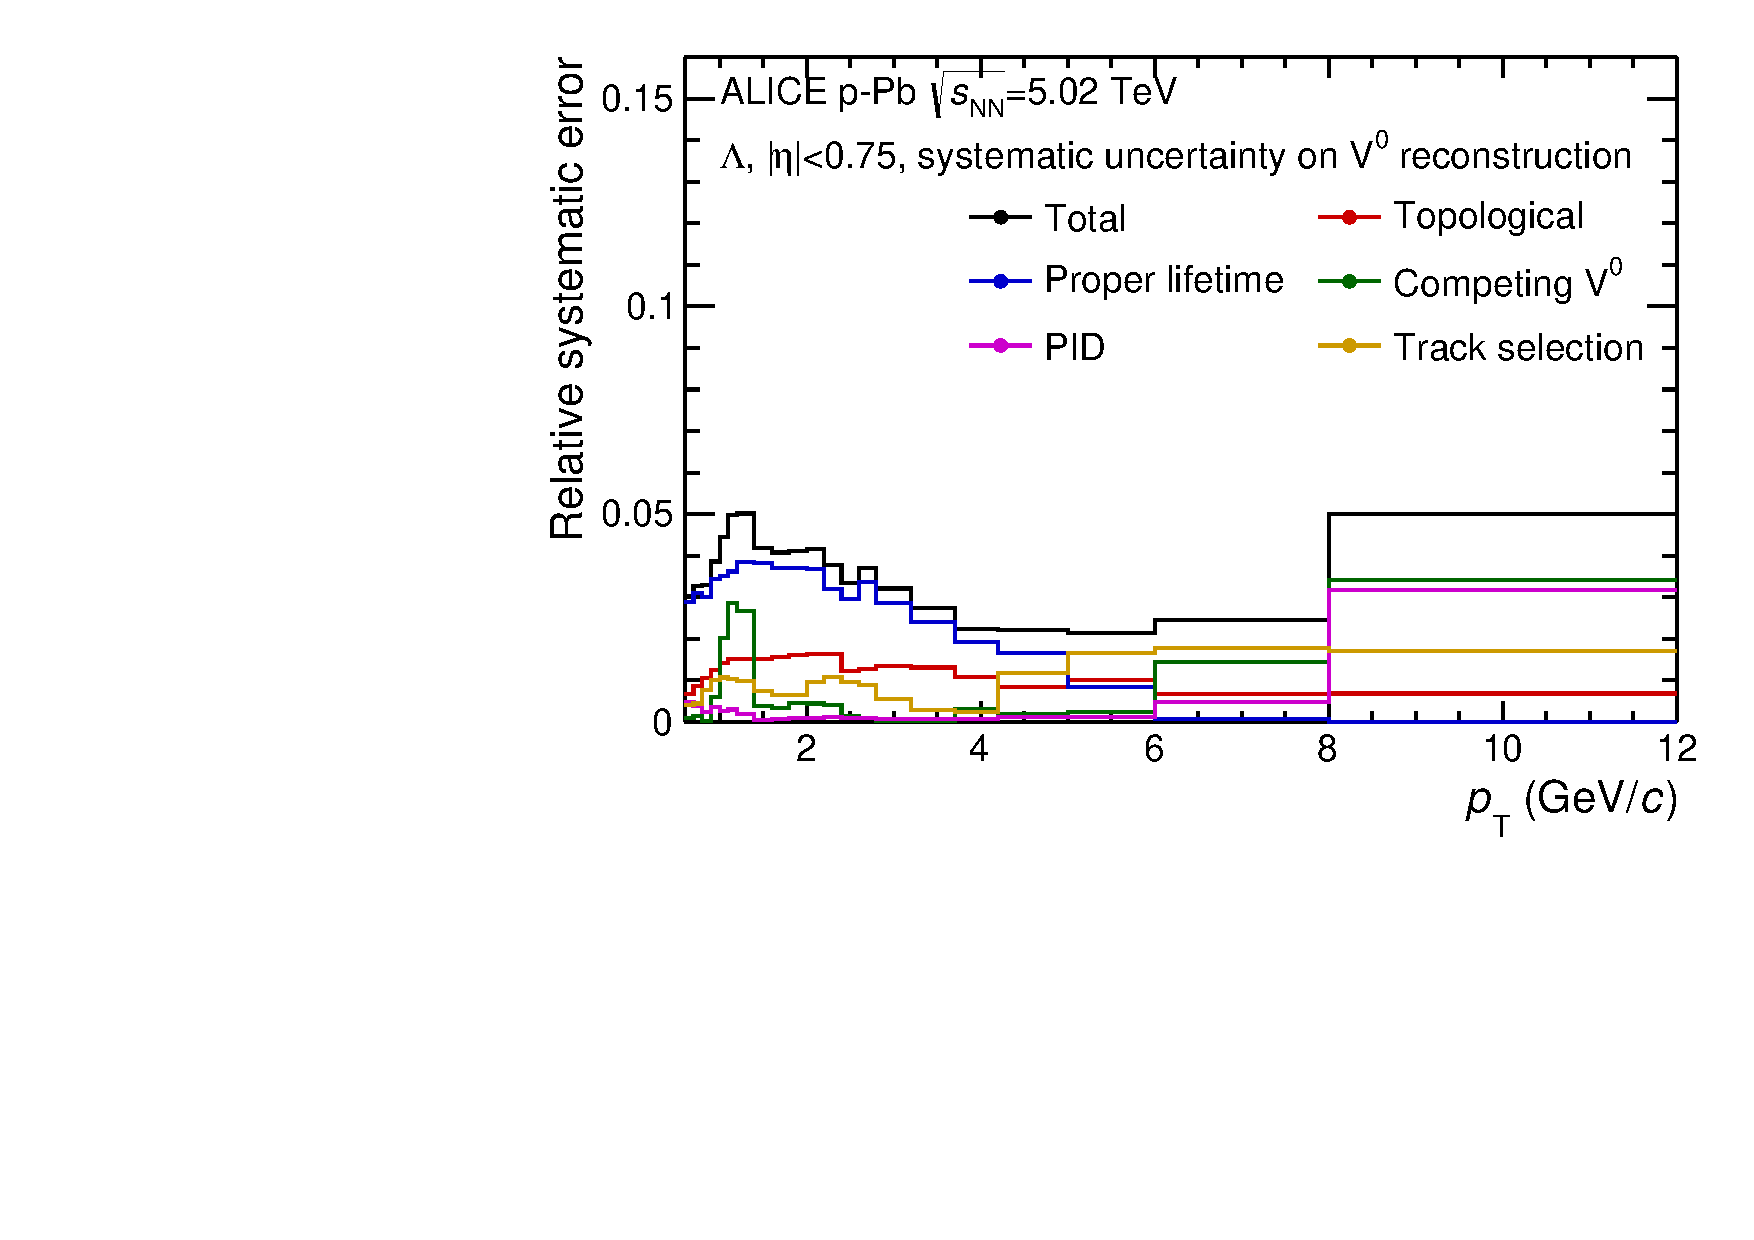
\includegraphics[width=.32\textwidth]{cSystIncl_Lambda}
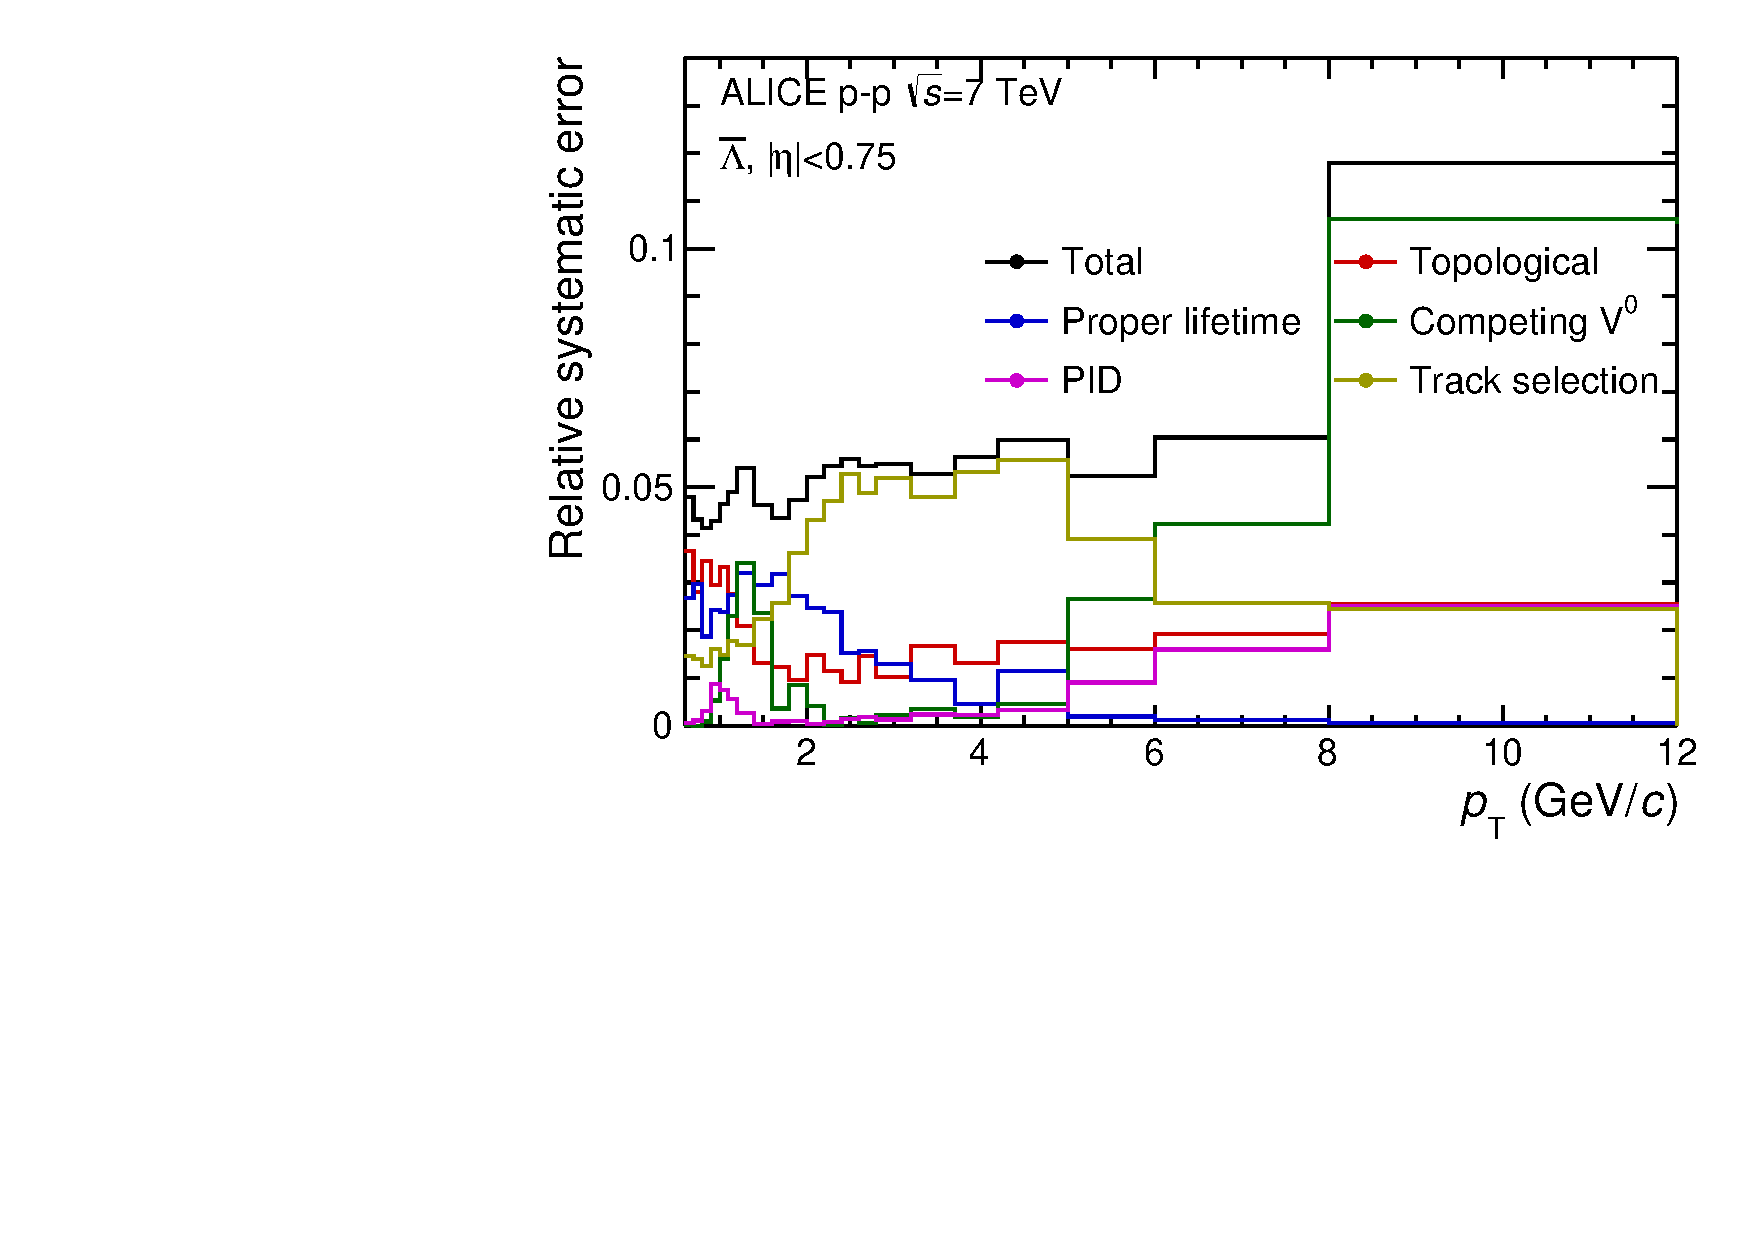
\includegraphics[width=.32\textwidth]{cSystIncl_AntiLa}
\caption{Systematic uncertainty of inclusive $\Vzero$s -- uncorrelated with statistics.}
\label{fig:c06SystInclV0s}
\end{center}
\end{figure}

\begin{figure}[t]
\begin{center}
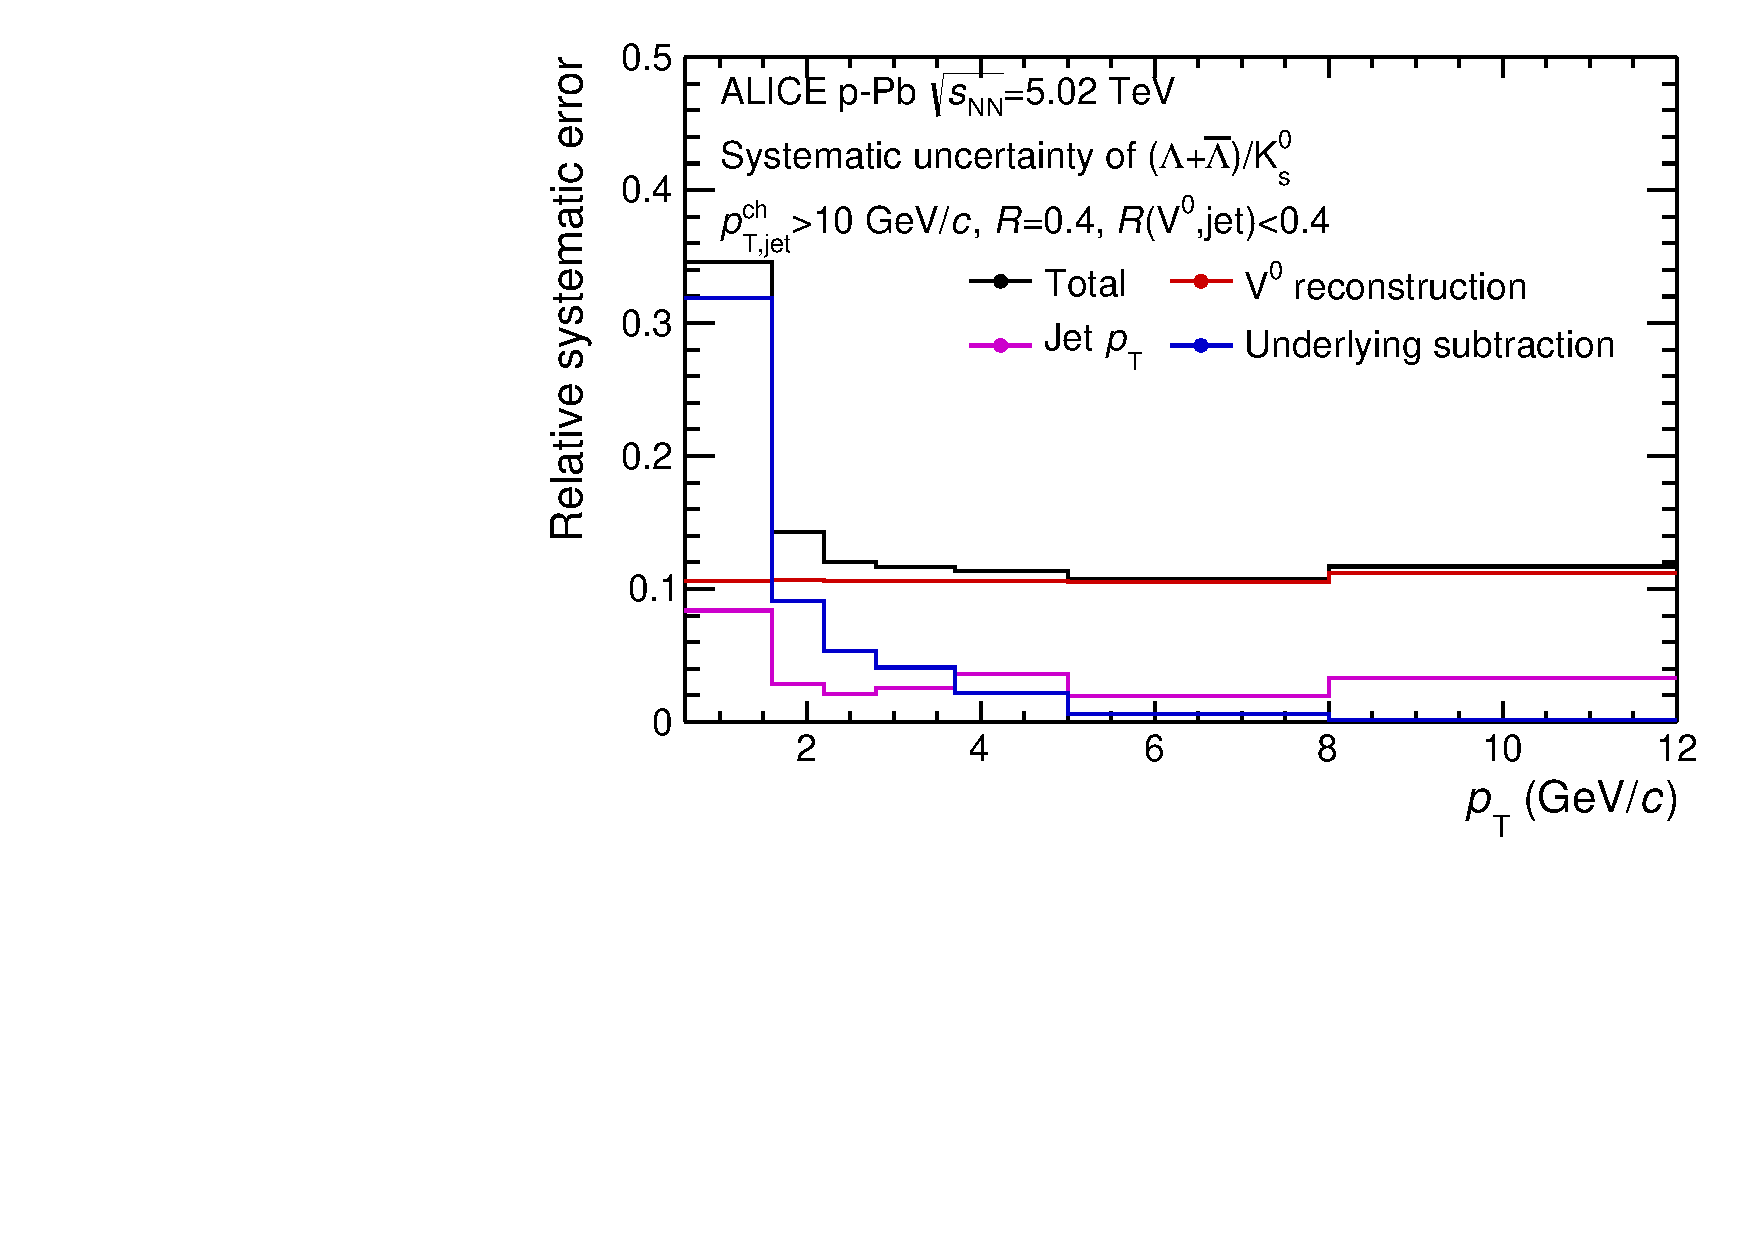
\includegraphics[width=.48\textwidth]{cSystInJE_RatioV_Ptj10}
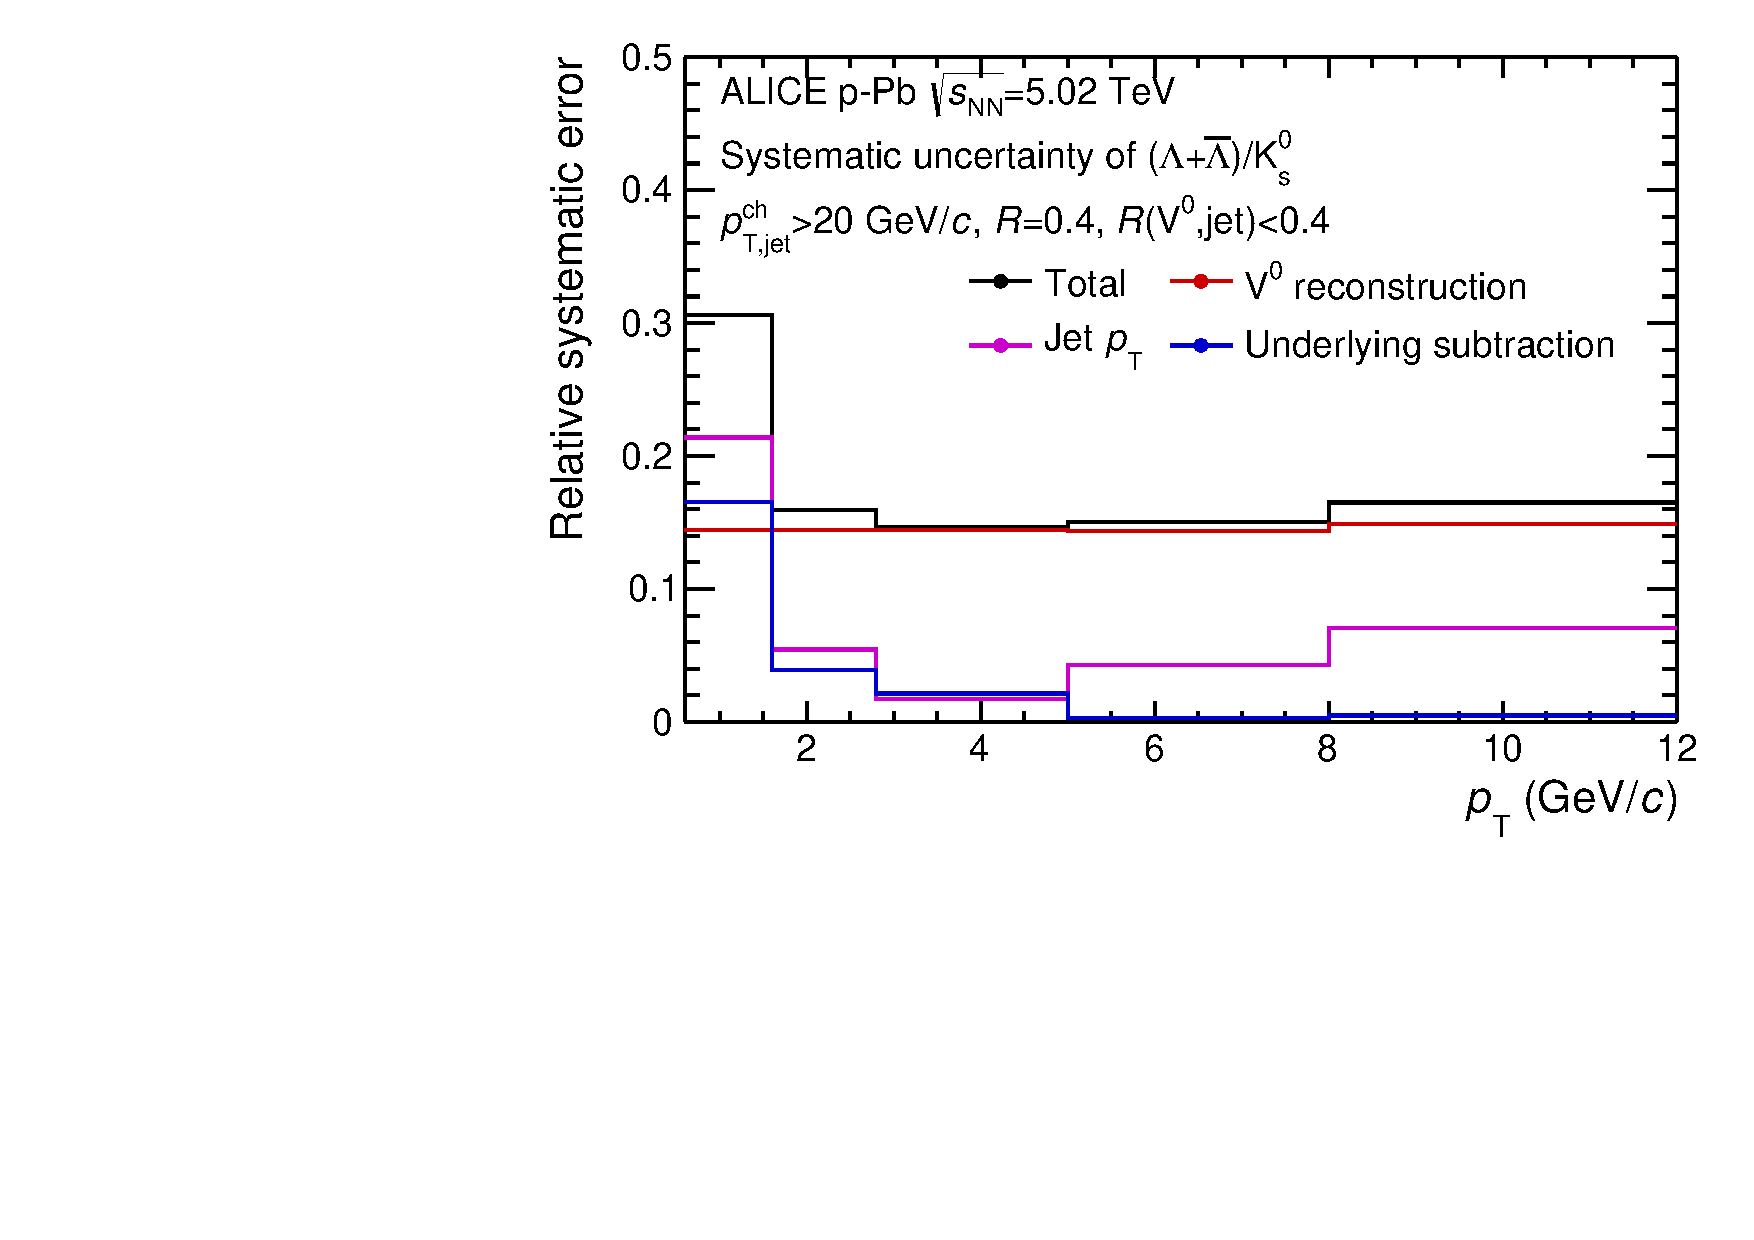
\includegraphics[width=.48\textwidth]{cSystInJE_RatioV_Ptj20}
\caption{Systematic uncertainty of $\Vzero$s in jets -- correlated with statistics.}
\label{fig:c06SystV0InJets}
\end{center}
\end{figure}

The systematic uncertainty includes two catalogs.

One is independent on different $\Vzero$ selections and is evaluated using inclusive $\Vzero$s.
The knowledge of detector materials resulting a $4\%$ uncertainty~\cite{Abelev:2013haa}.
Track and topology selections, up to $3\%$ ($5\%$) for $\Kshort$ ($\Lambda$ and $\AntiLa$) depend on $\pT$ (see~\cite{Abelev:2013xaa} for the details).
The systematic uncertainty on feed-down correction for $\Lambda$ and $\AntiLa$ was used the spread of the feed-down fractions determined for different event multiplicity ranges with respect to the minimum bias events is $5\%$ ($7\%$) in $\pT<3.7~\GeVc$ ($<3.7~\GeVc$)~\cite{Abelev:2013haa}.
For the JC selection, an extra $5\%$ \ask{(to be checked)} uncertainty was added in $\pT<6~\GeVc$ for the discrepancy between \textsc{Pythia} interpolations and the values for inclusive $\Lambda$ and $\AntiLa$.

\begin{table}[t]
\centering 
\begin{tabular*}{\linewidth}{@{\extracolsep{\fill}}lccc}
\hline
&&&\\[-0.7em]
 & $\Kshort$ & \multicolumn{2}{c}{$\Lambda$($\AntiLa$)}\\[0.3em]
\hline
&&&\\[-0.7em]
Proper lifetime & 2\% & \multicolumn{2}{c}{2\%} \\[0.3em]
Material budget & 4\% & \multicolumn{2}{c}{4\%} \\[0.3em]
Track selection  & 4\% & \multicolumn{2}{c}{4\%} \\[0.3em]
TPC PID & 1\% & \multicolumn{2}{c}{1\%} \\[0.3em]
Multiplicity & \multirow{2}{*}{2\%} & \multicolumn{2}{c}{\multirow{2}{*}{2\%}} \\
dependence & & \\[0.3em]
\hline
\hline
&&&\\[-0.7em]
\pT\ (\GeVc)  &  & $<$ 3.7 & $>$ 3.7\\[0.3em]
\hline
&&&\\[-0.7em]
Feed-down  &  & \multirow{2}{*}{5\%} & \multirow{2}{*}{7\%}\\
correction & & &\\[0.3em]
    \hline
    \hline
    &&&\\[-0.7em]
\pT\ (\GeVc)  &  & $<$ 3.7 & $>$ 3.7\\[0.3em]
    \hline
    &&&\\[-0.7em]
    Total & 6.5\% & 8\% & 9.5\% \\[0.3em]
\hline
\end{tabular*}
\caption{Main sources of systematic uncertainty for the $\Kshort$ and $\Lambda$($\AntiLa$).} \label{tab:v0syst}
\end{table}

In another catalog, the uncertainty on signal extraction, is depend on the various of $\Vzero$ selections.
As shown in section~\ref{sec:V0Reco}, to subtract the combinatory background via the bin counting approach, the signal region and sidebands are defined in $[-N\sigma,N\sigma]$ and, $[-2N\sigma,-N\sigma]$ and $[N\sigma,2N\sigma]$, respectively, where $\sigma$ is the $\pT$-dependent mass resolution, nominal $N=6$.
The $\pT$-dependent uncertainty on signal extraction is estimated by choosing the maximal deviation between varied $N$ in $4$, $5$ and $7$ and nominal spectra values obtained in each $\pT$ bin.
Since the bin counting fit is sensitive the statistic of $\Vzero$ candidates, this uncertainty is evaluated for each individual $\Vzero$ selection. \ask{-- Cite values, table or figure?}

There are two additional uncertainty sources for $\Vzero$s associated to the hard scatterings: the jet $\pT$ resolution and underlying event subtraction.
The applied jet $\pT$ threshold was smeared by local background fluctuations and detector response and, resulted a $\sim 20\%$ resolution independent on jet $\pT$~\cite{Adam:2015hoa}.
The analysis was repeated with varying the jet $\pT$ threshold within $20\%$\footnote{$e.g.$ for $\pT[jet]>10~\GeVc$ ($20~\GeVc$), the analysis was repeated in $\pT[jet]>8~\GeVc$ ($16~\GeVc$) and $\pT[jet]>12~\GeVc$ ($24~\GeVc$).} to evaluate the uncertainty on jet $\pT$ resolution.
For the underlying event subtraction, the PC selection was used as the default underlying event estimator, while the uncertainty was given using the OC with $R_{\rm cut}=0.6$ and NJ selections.
Each of these uncertainty source was evaluated as the $\pT$-dependent standard deviation between varied and nominal $\pT$-spectra values in each bin.
They were added in quadrature together with other uncertainties to yield the overall systematic uncertainty on the $\pT$ spectra.
Since these uncertainties are correlated for the $\Kshort$ and $\Lambda$ ($\AntiLa$) spectra and do partly cancel in the $\Lambda/\Kshort$ ratios.
In this case, they were evaluated by dividing $\Lambda$ ($\AntiLa$) and $\Kshort$ spectra obtained with the same selection variations.
